% \begin{document}

\chapter{Matroids and Matroid Intersections}

\section{Matroids}
\subsection{Greedy Algorithm for Max Weight Spanning Trees}

Let's start by getting a better understand perhaps the easiest of algorithms: always select the
best available option in a greedy way. We first describe the algorithm when considering the
spanning tree problem or rather the maximum weight forest problem. First recall the definition
of the maximum weight spanning tree problem:\footnote{It is perhaps more common to consider the
minimum spanning tree problem (which is equivalent by replacing each weight $w(e)$ by $-w(e)$).
Here we consider the maximum weight spanning tree problem for the purpose of generalizing it to
matroids.}

\dfn{Max Weight Spanning Trees}{
Given a connected undirected graph $G=(V,E)$ with edge weights $w:E\to\mathbb{R}$, find a
spanning tree $T\subseteq E$ of maximum total weight $w(T) := \sum_{e\in T} w(e)$.
}

\ex{}{
The following undirected edge-weighted graph has two maximum spanning trees:
$\{\{A,B\},\{B,C\},\{B,D\}\}$ and $\{\{A,C\},\{B,C\},\{B,D\}\}$.

\begin{center}
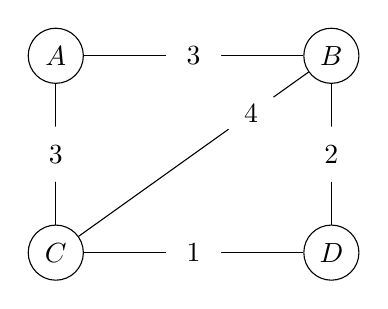
\begin{tikzpicture}[every node/.style={circle,draw,minimum size=7mm,inner sep=0pt}]
  \node (A) at (0,2.5) {$A$};
  \node (B) at (3.5,2.5) {$B$};
  \node (C) at (0,0) {$C$};
  \node (D) at (3.5,0) {$D$};
  \draw (A) -- node[draw=none,fill=white,midway] {3} (B);
  \draw (A) -- node[draw=none,fill=white,midway] {3} (C);
  \draw (B) -- node[draw=none,fill=white,near start] {4} (C);
  \draw (B) -- node[draw=none,fill=white,midway] {2} (D);
  \draw (C) -- node[draw=none,fill=white,midway] {1} (D);
\end{tikzpicture}
\end{center}
}

We are now going to describe the most basic greedy algorithm there is: repeatedly add the edge of
largest weight that does not create a cycle. When considering the spanning tree problem this is
known as Kruskal's algorithm (named after its inventor).

\bigskip
\noindent\fbox{\parbox{0.95\textwidth}{
\textbf{\Greedy$(G,w)$:}\\[2pt]
\textbf{Input:} A connected undirected graph $G=(V,E)$ and weights $(w_e)_{e\in E}$.\\
\textbf{Output:} A maximum weight spanning tree $S$.
\begin{enumerate}[leftmargin=2em,label=\arabic*.]
  \item Sort and relabel the edges so that $w_{e_1}\ge w_{e_2}\ge\cdots\ge w_{e_{|E|}}$.
  \item $S\leftarrow\emptyset$.
  \item \textbf{for} $i=1$ \textbf{to} $|E|$:
  \item \hspace{1em}\textbf{if} $S+e_i$ is acyclic \textbf{then} $S\leftarrow S+e_i$.
  \item \textbf{return} $S$.
\end{enumerate}
}}
\bigskip

\paragraph{Runtime analysis.}
Steps 3--4 can be implemented in almost linear time using the \textsc{Union-Find} (also called
\textsc{Disjoint-Set}) data structure that I hope you have seen during your Bachelor studies.
The running time is thus dominated by the sorting of Step 1. Using e.g.\ Merge-Sort this step
runs in time $\Theta(|E|\log|E|)$. The total running time is thus $\Theta(|E|\log|E|)$.

\paragraph{Why does it work?}
The correctness of the algorithm follows from the following lemma.

\mlenma{}{\label{lem:greedy}
\Greedy{} returns a maximum-weight spanning tree.
}

\pf{}{
Suppose not. Let $S=\{s_1,s_2,\ldots,s_{n-1}\}$ be the set (spanning tree) returned by the
algorithm and suppose that a solution $T$ has a higher weight, where
$T=\{t_1,t_2,\ldots,t_{n-1}\}$ (indexed in decreasing weight). Let $p$ be the first index such
that $w(t_p)>w(s_p)$. Let $A=\{t_1,\ldots,t_p\}$ and $B=\{s_1,\ldots,s_{p-1}\}$. Now we have
the following key property of acyclic graphs.

\medskip
\noindent\textbf{Key property:} As $|A|>|B|$, there exists $e\in A\setminus B$ such that $B+e$
is acyclic.

\medskip
The key property follows from that an acyclic graph with $k$ edges has $n-k$
components.\footnote{It is a good exercise to prove this using induction!} Thus the graph
$(V,A)$ has fewer components than $(V,B)$ and so at least one edge $e\in A$ must connect two
different components of $(V,B)$. It follows that $e\notin B$ and that $B+e$ is acyclic.

Having proved the key property, we conclude as follows. Since $w(e)\ge w(t_p)>w(s_p)$, $e$
should have been selected when it was considered.

To be more precise and detailed, when $e$ was considered, the greedy algorithm checked whether
$e$ could be added to the current set at the time, say $B'$. But since $B'\subseteq B$, adding
$e$ to $B'$ would have resulted in an acyclic graph (a subset of acyclic edges is also acyclic)
since its addition to $B$ results in an acyclic graph.

This gives a contradiction and completes the proof.
}

\subsection{Matroids and Greedy}

Note that in the correctness of the \Greedy{} algorithm for max-weight spanning trees
(Lemma~\ref{lem:greedy}) we used two properties of acyclic graphs: (i) a subset of acyclic edges
is acyclic and (ii) for two acyclic edge sets $A,B$ on the same vertex-set with $|A|>|B|$ there
is $e\in A\setminus B$ such that $B+e$ is acyclic.

Matroids are defined to satisfy these two properties and we will see that they define the set of
problems for which the basic greedy algorithm works. It also generalizes the notion of linear
independence in matrices. There are many equivalent definitions. We use the one that focus on its
independent sets.

\dfn{Matroid}{
A matroid $M=(E,\mathcal{I})$ is defined on a finite ground set $E$ and a family $\mathcal{I}$ of
subsets of $E$ that are called independent sets satisfying two axioms:
\begin{description}[leftmargin=3em,style=nextline]
  \item[(I1)] if $X\subseteq Y$ and $Y\in\mathcal{I}$ then $X\in\mathcal{I}$.
  \item[(I2)] if $X\in\mathcal{I}$ and $Y\in\mathcal{I}$ and $|Y|>|X|$ then
    $\exists e\in Y\setminus X: X\cup\{e\}\in\mathcal{I}$.
\end{description}
}

\noindent Remarks:
\begin{itemize}
  \item Letting $E$ be the edges of a graph and $\mathcal{I}=\{F\subseteq E: F \text{ is acyclic}\}$
    defines a so-called \emph{graphic matroid}. Note that it satisfies (I1) since the subset of an
    acyclic set of edges is acyclic and it satisfies (I2) due to the key property used in the proof
    of Lemma~\ref{lem:greedy}. We see more examples of matroids in Section~\ref{sec:examples}.
  \item The family $\mathcal{I}$ may be exponential in the size of the ground set $E$ (as is the
    case for example for graphic matroids of complete graphs). One therefore often assumes that
    $\mathcal{I}$ is given implicitly by having a \emph{membership oracle}: an algorithm that given
    $I\subseteq E$ efficiently answers whether $I\in\mathcal{I}$.
\end{itemize}

\dfn{Matroid Base}{
  A \textit{base} of a matroid is an independent set of maximum cardinality.
}

\clm{Maximality of bases}{}{
  All maximal independent sets are bases and have the same cardinality.
}

\pf{}{
  Implied by the second axiom.
}

With the more abstract notation of matroids, the basic greedy algorithm becomes

\bigskip
\noindent\fbox{\parbox{0.95\textwidth}{
\textbf{\Greedy$(M,w)$:}\\[2pt]
\textbf{Input:} A matroid $M=(E,\mathcal{I})$ and weights $(w_e)_{e\in E}$.\\
\textbf{Output:} A maximum weight base $S$.
\begin{enumerate}[leftmargin=2em,label=\arabic*.]
  \item Sort and relabel the elements so that $w_1\ge w_2\ge\cdots\ge w_{|E|}$.
  \item $S\leftarrow\emptyset$.
  \item \textbf{for} $i=1$ \textbf{to} $|E|$:
  \item \hspace{1em}\textbf{if} $S+i\in\mathcal{I}$ \textbf{then} $S\leftarrow S+i$.
  \item \textbf{return} $S$.
\end{enumerate}
}}
\bigskip

The concept of matroids was defined so as to enable the correctness analysis of the basic greedy
algorithm. Perhaps more surprisingly, it is if and only if.

\thm{Rado'57/Gale'68/Edmonds'71}{\label{thm:main}
For any ground set $E=\{1,2,\ldots,n\}$, and a family of subsets $\mathcal{I}$, \Greedy{} finds a
maximum weight base for
any set of weights $w:E\to\mathbb{R}$ if and only if $M=(E,\mathcal{I})$ is a matroid.
}

The if direction ($\Leftarrow$ part) follows from Lemma~\ref{lem:greedy}. For the only if direction
we have the following claim.

\label{claim:onlyif}
\clm{$\Rightarrow$ part}{}{
Suppose $(E,\mathcal{I})$ is not a matroid. There exists an assignment of weights $w:E\to\mathbb{R}$
so that \Greedy{} does not return a maximum weight base.
}

\pf{}{
If $(E,\mathcal{I})$ is not a matroid, then it violates at least one of the two axioms.

First suppose $\mathcal{I}$ is not a downward-closed family of sets, i.e., it violates (I1).
Therefore, there exist two sets $S\subset T$ such that $S\notin\mathcal{I}$ and $T\in\mathcal{I}$.
Consider the following weights:
\[
  w_i =
  \begin{cases}
    2 & i\in S,\\
    1 & i\in T\setminus S,\\
    0 & \text{otherwise.}
  \end{cases}
\]
By the weight assignment, the algorithm first considers the elements of $S$, then the elements of
$T$, and then the rest of the elements. Suppose the algorithm selects a subset $S_1$ of $S$. Since
$S\notin\mathcal{I}$, $S_1$ is a strict subset. Out of the remaining elements the algorithm can
select at most $T\setminus S$. So the weight of the independent set that the algorithm returns is
at most $2|S_1|+|T\setminus S|$ which is less than $w(T)$ so it is not a maximum weight independent
set.

Second suppose that the extension axiom is violated (but downwardness is satisfied). In particular,
let $S,T\in\mathcal{I}$ be two independent sets such that $|S|<|T|$, and for all $i\in T\setminus S$,
$S+i\notin\mathcal{I}$. Now use the following weights
\[
  w_i =
  \begin{cases}
    1+\frac{1}{2|S|} & i\in S,\\
    1 & i\in T\setminus S,\\
    0 & \text{otherwise.}
  \end{cases}
\]
Because of downwardness the algorithm would select all elements in $S$ and return an independent
set of value $|S|+1/2$ where as the optimal set would have value at least $|T|>|S|+1/2$.
}

\subsection{Examples of matroids}\label{sec:examples}

We already saw the graphic matroids. Other basic matroids are as follows:

\subsubsection{$k$-Uniform matroid}

A matroid $M=(E,\mathcal{I})$ is $k$-Uniform if $\mathcal{I}$ satisfies:
\[
  \mathcal{I}=\{X\subseteq E: |X|\le k\}.
\]

\subsubsection{Partition matroid}

A matroid $M=(E,\mathcal{I})$ is a partition matroid if $E$ is partitioned into disjoint sets
$E_1,E_2,\ldots,E_\ell$ and
\[
  \mathcal{I}=\{X\subseteq E: |E_i\cap X|\le k_i \text{ for } i=1,2,\ldots,\ell\}.
\]

\subsubsection{Linear matroid}

A matroid $M=(E,\mathcal{I})$ is a linear matroid when it is defined from a matrix $A$. Let $E$ be
the index set of the columns and for $X\subseteq E$ let $A_X$ be the matrix consisting of the
columns indexed by $X$. Define $\mathcal{I}$ by
\[
  \mathcal{I}=\{X\subseteq E: \operatorname{rank}(A_X)=|X|\}.
\]

\subsubsection{Truncated matroid}

A truncated matroid $M_k=(E,\mathcal{I}_k)$ is defined from a matroid $M=(E,\mathcal{I})$ such that
\[
  \mathcal{I}_k=\{X\in\mathcal{I}: |X|\le k\}.
\]
It is quite easy to verify that the axioms still hold for $M_k$, as $X\in\mathcal{I}_k$ implies
$X\in\mathcal{I}$ for all $X\subseteq E$.

(I1) holds because $B\in\mathcal{I}_k$ means that $|B|\le k$ and $A\subseteq B$ thus means
$|A|\le k$ as well. We know that $M$ is a matroid so (I1) holds for $M$, which implies
$A\in\mathcal{I}$. We conclude that $A\in\mathcal{I}_k$.

The same reasoning can verify (I2): if $A,B\in\mathcal{I}_k$ and $|B|>|A|$, then $|B|\le k$ and
$|A|\le k-1$. We know that (I2) holds for $M$, so the inclusion of $\mathcal{I}_k$ in $\mathcal{I}$
tells us that $\exists e\in B\setminus A$ such that $A+e\in\mathcal{I}$. The fact that
$|A+e|\le k-1+1=k$ allows us to conclude.

% \end{document}
